\chapter{Einleitung}
\label{chap:introduction}

%%%%%%%%%%%%%%%%%%%%%%%%%%%%%%%%%%%%%%%%%%%%%%%%%%%%%%%%%%%%
\section{Motivation}
\label{sec:introduction:motivation}
%%%%%%%%%%%%%%%%%%%%%%%%%%%%%%%%%%%%%%%%%%%%%%%%%%%%%%%%%%%%

Die GPS-Navigation ist seit Jahren aus keinem Auto mehr wegzudenken. Wo früher Karten genutzt wurden und nach Straßennamen geschaut wurde, wird heute die Zieladresse in das Navigationssystem eingegeben und das System bestimmt selbstständig die aktuelle Position, die Zielposition und errechnet die bestmögliche Route.
Ein Problem der GPS-Navigation ist jedoch, dass diese nur unter freiem Himmel akzeptabel funktioniert.
Da wir in der Realität jedoch den Großteil unserer Zeit in Gebäuden aufhalten, ist der GPS-Ansatz dort wenig hilfreich.

Daher ist es sinnvoll, eine Alternative zu GPS zu schaffen, welche diese Funktionen in Innenräumen realisiert.
Da man jedoch für Innenräume kein eigenes Navigationssystem kaufen möchte, liegt die Idee nah, diese Konzept auf einem Gerät zu realisieren, welches viele Menschen schon besitzen und auch für die GPS-Navigation nutzen. 
Das Smartphone.

In Abbildung 1 ist zu erkennen, wie die Verbreitung der Smarthphones in den letzten Jahren sehr stark zugenommen hat. Dadurch kann man annehmen, dass ein Großteil der potentiellen Nutzer der Indoor Positionierung auch ein Smartphone besitzen.
\begin{figure}[htb]
	\centering
		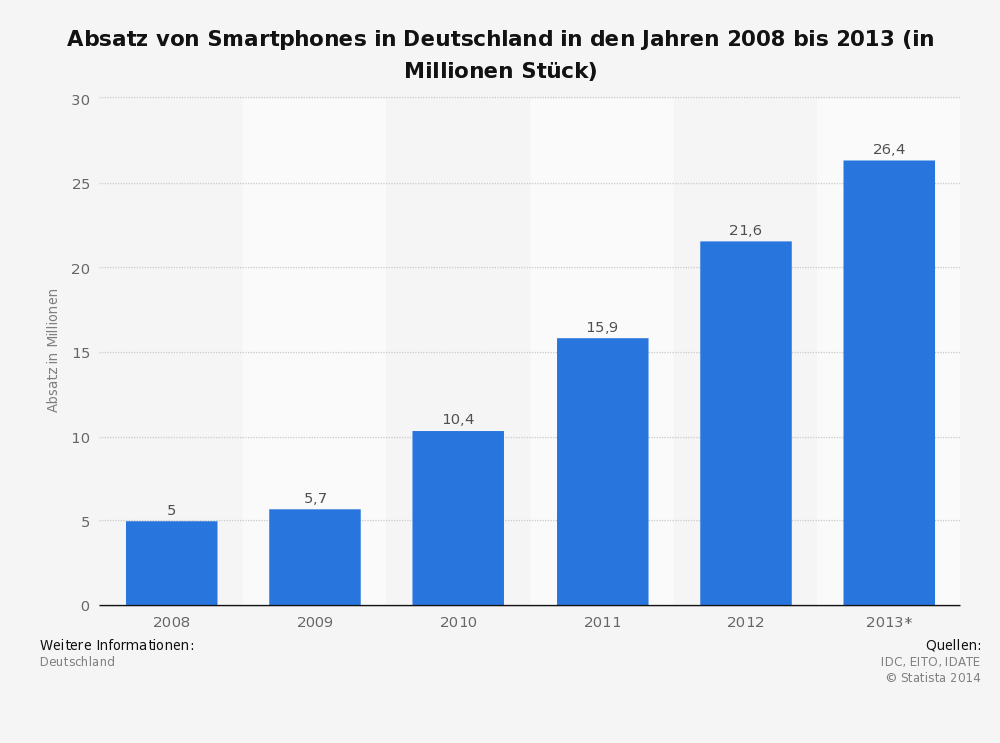
\includegraphics[height=8cm]{pictures/statistik-smartphonenutzung.png}
		\caption{Smartphoneabsatz in Deutschland}
\end{figure}

Für die Realisierung der Indoor Positionierung kommen verschiedene Technologien in Frage. Darunter zum Beispiel Wireless LAN, RFID oder Bluetooth.
Diese Technologien bieten sich an, da sie standardmäßig in vielen Smartphones integriert sind und so nicht der Zwang besteht ein neues Gerät oder eine Erweiterung zu kaufen.


Schlussendlich viel die Entscheidung der zu verwendenden Technologie auf Bluetooth, da dieses eine sehr hohe Verbreitung bietet und auch viele Vorteile mit sich bringt. Zum einen ermöglicht Bluetooth eine schnelle und einfache Einrichtung und zum anderen benötigen die Bluetooth-Sendestationen wenig Energie, sodass nicht zwingend einen Stromanschluss vorhanden sein muss, sondern auch einen Batteriebetrieb über mehrere Monate bis Jahre hinweg möglich ist.

Die Positionierung in Innenräumen mittels Bluetooth ist ein relativ neuer Ansatz, welcher jedoch seit der Präsentation von Bluetooth Low Energy und der Vorstellung der iBeacons-Technologie von Apple immer mehr an Aufmerksamkeit gewonnen hat. So setzt zum Beispiel Apple selbst die iBeacons-Technologie in ihren Geschäften ein, um dem Kunden gezielte Werbung zu den in der Nähe befindlichen Produkten zu bieten.

%%%%%%%%%%%%%%%%%%%%%%%%%%%%%%%%%%%%%%%%%%%%%%%%%%%%%%%%%%%%
\section{Ziele der Bachelorarbeit}
\label{sec:introduction:goal}
%%%%%%%%%%%%%%%%%%%%%%%%%%%%%%%%%%%%%%%%%%%%%%%%%%%%%%%%%%%%


Das Hauptziel dieser Arbeit ist es zu untersuchen, in wie weit sich Bluetooth Low Energy, beziehungsweise die darauf basierende iBeacons-Technologie, für eine akzeptable Indoor Positionierung eignen, um Endgeräte zum Beispiel in Verkaufsräumen zu orten und zu identifizieren.

Dabei soll bestimmt werden, welches Verfahren sich am Besten für die Positionierung in Innenräumen eignet und ob es Unterschiede zwischen verschiedenen Sende- und auch Empfangsgeräten gibt.

Für diese Tests werden ausschließlich Apple-Geräte genutzt, da hier eine übersichtlichere Auswahl auf dem Markt herrscht, sodass die Basis der zu nutzenden Geräte überschaubar bleibt und nur wenige Geräte getestet werden müssen. Ein weiterer Grund ist, dass iOS, das Betriebssystem des Apple iPhone und iPads, bisher das einzige mobile Betriebssystem ist, welches die iBeacons-Technologie offiziell und nativ unterstützt.

Im Laufe der Bachelorarbeit soll deshalb eine iOS-Applikation entwickelt werden, welche eine Positionierung in einem Innenraum implementiert. Dabei wird die von Apple bereitgestellte CoreLocation-API genutzt, welche die Verarbeitung der iBeacon-Daten übernimmt. Die genutzten iBeacon-Sender kommen von Drittherstellern und sind derzeit noch in einem Vorserienstadium. 

Zum Abschluss soll eine grundlegende Positionierung, eine Anzeige der aktuellen Position auf eine Karte und das Auslösen bestimmter Aktionen an festgelegten Orten implementiert sein.



